\section{Agent Crews}\label{sec:agents}
In this section we will describe the five agents crews of our model:
\begin{enumerate}
    \item Emergency Services.
    \item Firefighters.
    \item Medical Services.
    \item Forensics Team.
    \item Public Communications.
\end{enumerate}
We will discuss the main tasks, tools, types, and properties of each agent that comprises the crews. Figure \ref{fig:diagram} illustrates the interactions between crews of agents as well as among agents within the different crews. Communication between crews is carried out through a communication channel, which only one agent per crew has access to.

\begin{figure}[H]
\centering
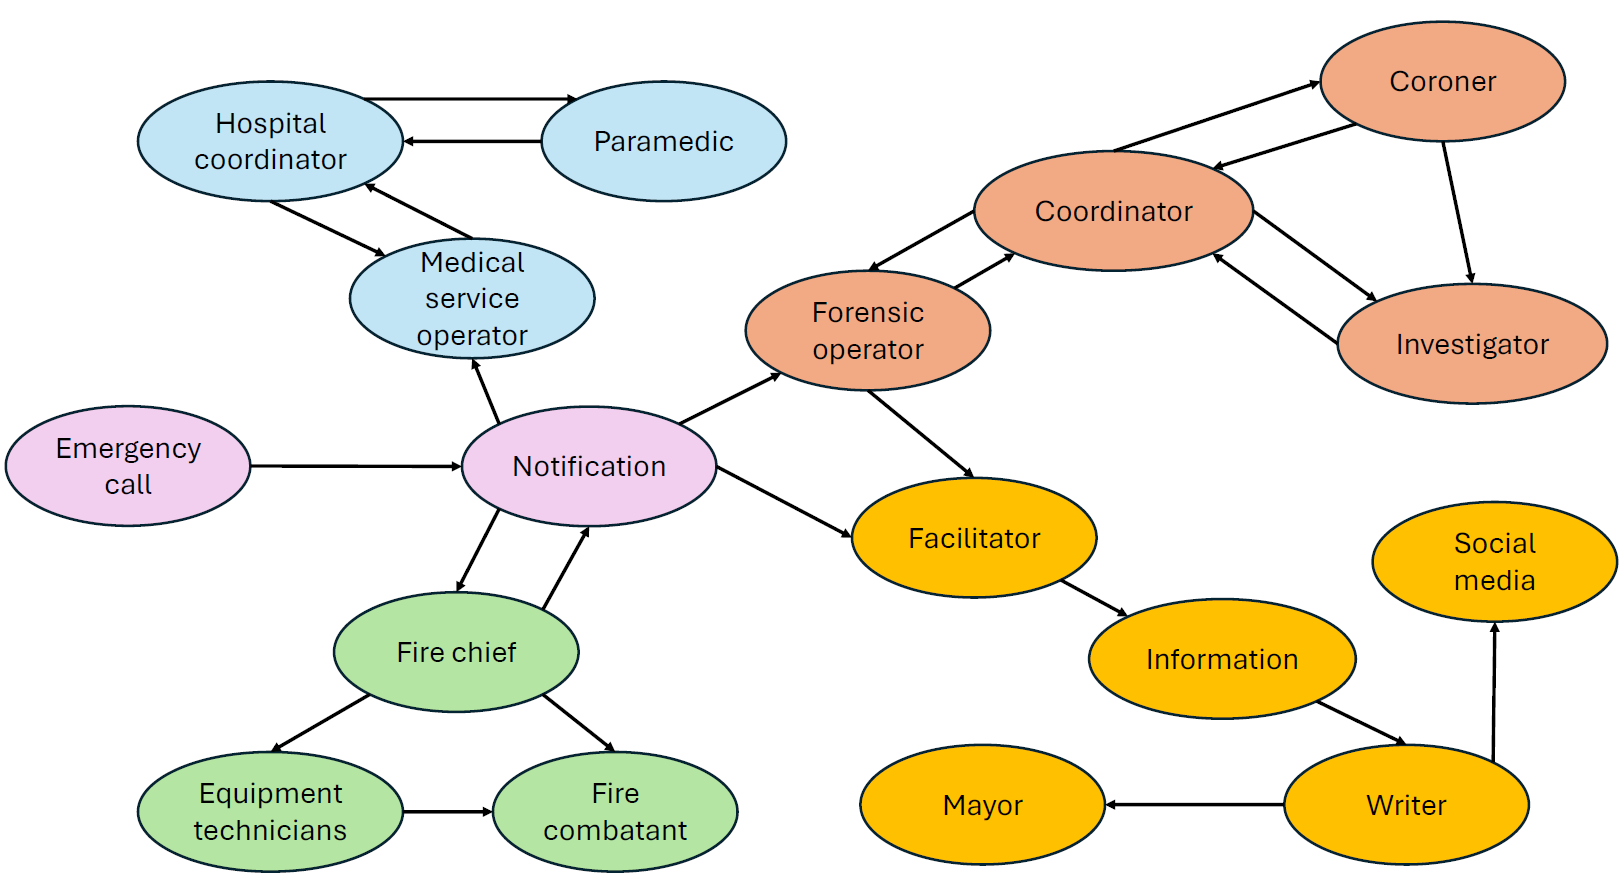
\includegraphics[width=0.6\textwidth]{../figures/diagram_between_agents.png}
\caption{Diagram of the interaction between the crews of agents and the agents within the different crews. Emergency services: purple, firefighters: green, medical services: blue, forensic team: red and public communication: orange.}
\label{fig:diagram}
\end{figure}

\subsection{Emergency Service Agent Crew}

This crew is responsible for handling emergency calls and coordinating communication responses with the appropriate teams.

\subsubsection{Emergency Call Agent}

The Emergency Call Agent serves as the main point of contact for incoming emergency calls, responsible for collecting essential information from the caller and assessing the severity and nature of the incident.

\begin{itemize}
    \item \textbf{Main task:} To receive, assess, and categorize emergency calls, and subsequently notify the appropriate response units.
    \item \textbf{Tools:} 
    \begin{itemize}
        \item \emph{Communication Software}:  A digital call-taking software to communicate with callers and to log the conversation.
        \item \emph{Data Entry Interface}: A computer system or software for systematically entering and recording emergency details.
        \item \emph{Incident Assessment Tools}: A map to quickly locate and verify the caller's position and assess the scene, potentially including software for prioritizing the severity of the incident if necessary.
    \end{itemize}
    \item \textbf{Type:} Interface agent: This agent emphasizes autonomy and learning to support users. In this case, the Emergency Call Agent acts as a user interface for emergency call handling, gathering caller input and making proactive decisions on incident categorization.
    \item \textbf{Properties:}
    \begin{itemize}
        \item \emph{Reactivity}:  The Emergency Call Agent continuously interacts with the environment (incoming calls) and rapidly assesses each situation to provide an appropriate response.
        \item \emph{Proactiveness}: While primarily reactive, the Emergency Call takes initiative by categorizing and prioritizing incidents, ensuring the most urgent cases receive immediate attention.
        \item \emph{Social Ability}: Capable of basic communication with other agents and potentially human responders, using a structured communication protocol for efficient incident coordination.
        \item \emph{Autonomy}: Operates independently once set up, requiring minimal external input to manage call processing and categorization.
    \end{itemize}
\end{itemize}

\subsubsection{Notification Agent}

A bridge agent that ensures timely and accurate transmission of information between the Emergency Call Agent and emergency response teams.

\begin{itemize}
    \item \textbf{Main task:} To relay details about the incident to the respective emergency teams and manage ongoing updates throughout the response.
    \item \textbf{Tools:}
    \begin{itemize}
        \item \emph{Communication protocols}: Passes the information collected by the Emergency Call Agent to the appropriate teams (firefighters or medical services).
        \item \emph{Notification system}: Continues to relay new updates or details as they come in, ensuring no one is left out of important updates.
    \end{itemize}
    \item \textbf{Type:} Facilitator agent: This type emphasizes communication and interaction, managing the connections and information flow between agents. The Notification Agent serves as the coordinator in the emergency response communication network.
    \item \textbf{Properties:}
    \begin{itemize}
        \item \emph{Reactivity}: Monitors changes from both Emergency Call inputs and emergency response team feedback, adjusting notifications and updates based on dynamic incident progress.
        \item \emph{Social Ability}: Engages in continuous communication with multiple agents in real-time, ensuring all parties are kept informed and aligned on incident status.
        \item \emph{Temporal Continuity}: Remains active throughout the duration of an incident, managing and providing updates until the situation is resolved.
        \item \emph{Flexibility}: Adapts to various communication protocols and priority levels, adjusting its actions according to the severity of the situation and the availability of response teams.
    \end{itemize}
\end{itemize}

\subsection{Firefighters}
This agent crew is responsible to move to the location of a fire and to extinguish the fire.
\newline The agents that are part of this crew are: a \textbf{fire chief}, one \textbf{equipment technician} and a team of \textbf{fire combatants}.

\subsubsection{Fire Chief}
Takes calls from the emergency services and reports back.

\begin{itemize}
    \item \textbf{Main task:} The fire chief receives a call from the emergency service operator and relays the information to its agent crew members. Once the firefighter crew arrives at the fire scene, the fire chief provides updates on the situation back to the emergency service operator.
    \item \textbf{Tools:}
    \begin{itemize}
        \item \textit{Communication Device}: A device for effective communication with the other crews.
    \end{itemize}
    \item \textbf{Type:} Facilitator agent.
    \item \textbf{Most relevant properties:}
    \begin{itemize}
        \item \textit{Flexibility:} The fire chief must be able to adapt to changing circumstances and new information, ensuring that the crew can respond effectively to dynamic situations on the fire scene.
        \item \textit{Reactivity:} The fire chief needs to respond promptly to incoming information and evolving conditions during emergencies, ensuring that the crew is informed and can adjust their actions accordingly.
        \item \textit{Social Ability:} Effective communication and collaboration with both the emergency service operator and other crews are crucial for the fire chief to facilitate coordination and ensure that all parties are updated on the situation.
    \end{itemize}
\end{itemize}

\subsubsection{Equipment Technician}
Manages material required to extinguish a fire.

\begin{itemize}
    \item \textbf{Main task:}  Based on the information received from the fire chief, the equipment technician needs to determine which materials are necessary, such as fire hoses, personal protective equipment (PPE), and fire extinguishers, and packs these items and loads them on the fire truck before the agent crew moves to the location of the fire. It is crucial that sufficient materials are packed to ensure a safe and effective response.
    \item \textbf{Tools:}
    \begin{itemize}
        \item \textit{Material Management Software}: Has a database of all the available material, which can be modified when resources are used for the emergencies.
    \end{itemize}
    \item \textbf{Type:} Information agent.
    \item \textbf{Most relevant properties:}
    \begin{itemize}
        \item \textit{Flexibility:} The agent must adapt to different emergency scenarios and equipment needs quickly.
        \item \textit{Reactivity:} The technician must respond promptly to changing conditions and requirements during firefighting operations.
        \item \textit{Rationality:} The agent needs to make logical decisions about what materials to prioritize and pack based on available information.
    \end{itemize}
\end{itemize}

\subsubsection{Firefighter}
Extinguishes the fire.

\begin{itemize}
    \item \textbf{Main task:} The firefighting combatants unload the required equipment from the fire truck at the fire scene. They then assess the most effective strategy to extinguish the fire by coordinating with their fellow firefighters.
    \item \textbf{Tools:}
    \begin{itemize}
        \item \textit{GPS}: Can access a real-time map of the city to locate the location of the incident and calculate the best route to get there.
    \end{itemize}
    \item \textbf{Type:} Collaborative agent.
    \item \textbf{Most relevant properties:}
    \begin{itemize}
        \item \textit{Reactivity:} This property is crucial as firefighting involves rapidly changing situations that require immediate responses to new developments, such as flare-ups or structural shifts.
        \item \textit{Proactiveness:} The combatant must anticipate potential challenges and take initiative in strategizing the best approach to extinguishing the fire, helping to prevent escalation and ensure successful outcomes.
        \item \textit{Social Ability:} Strong social ability is essential for effective teamwork, enabling the combatant to communicate and collaborate with fellow firefighters to coordinate efforts and ensure safety.
    \end{itemize}
\end{itemize}

% Medical Services - Figure 1
\begin{frame}{Medical Services Process}
    \centering
    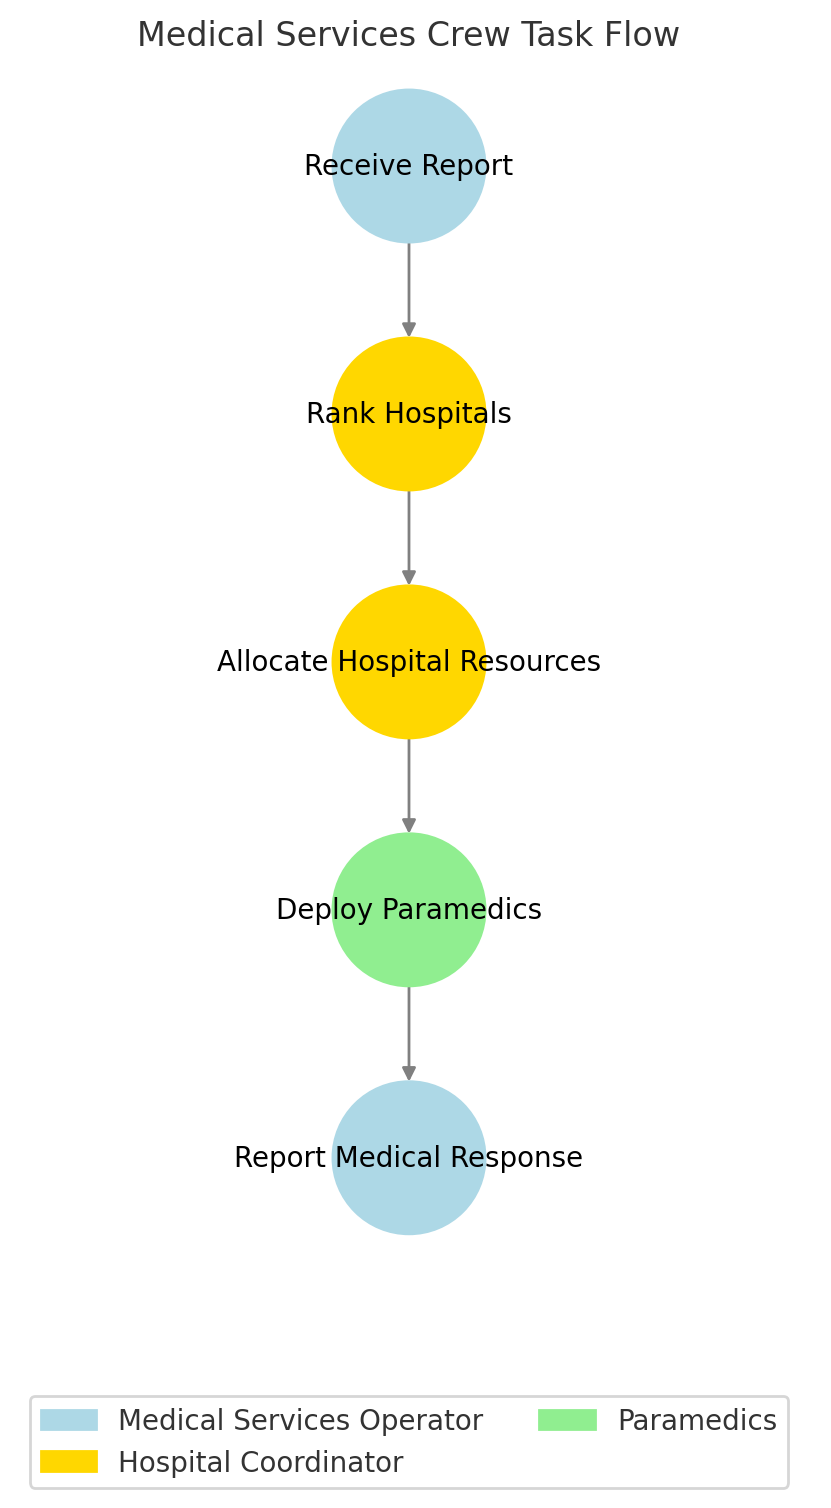
\includegraphics[height=\textheight]{figures/Medical_Services_Crew_Flow.png} 
\end{frame}

% Medical Services - Figure 2
\begin{frame}{Medical Services Outputs}
    \centering
    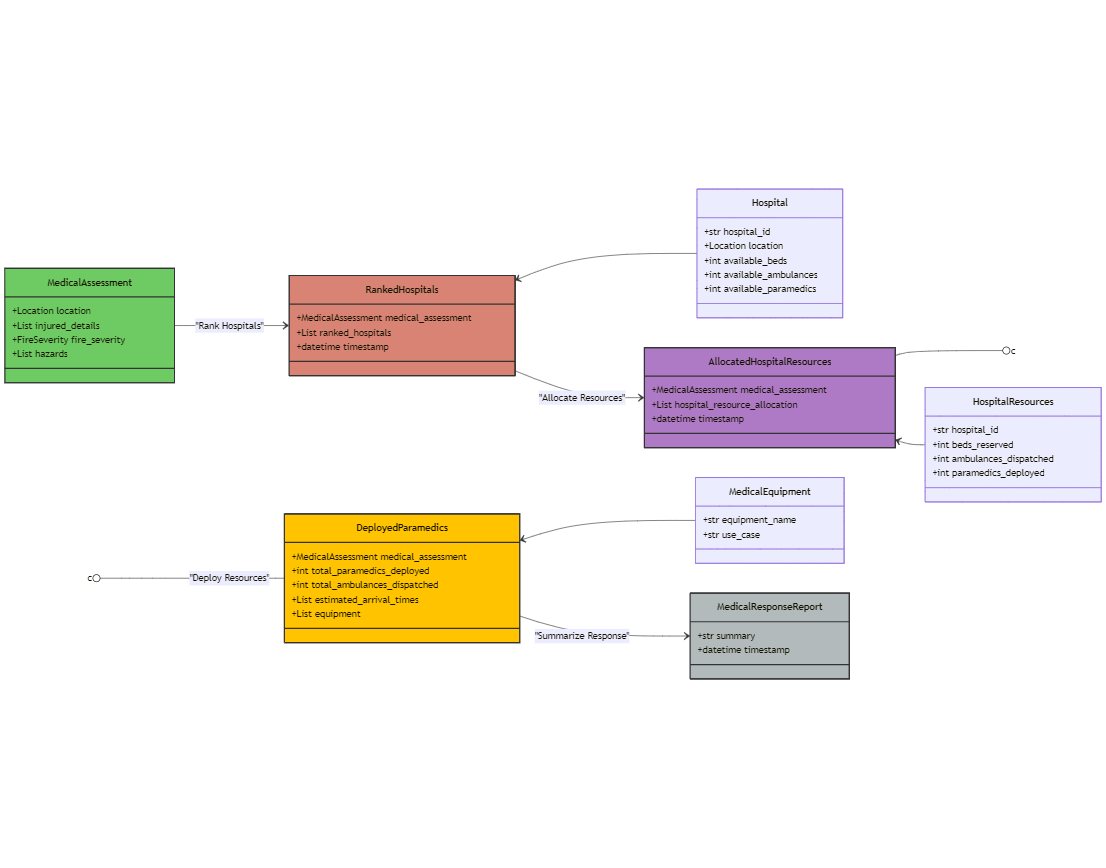
\includegraphics[width=\textwidth]{figures/MedicalServices_ClassDiagram.png}
\end{frame}
% Forensics Team
\subsection{Forensics Team}
\begin{frame}{Forensics Team}
    \begin{itemize}
        \item \textbf{Forensics Operator}:
        \begin{itemize}
            \item \alert{Facilitator} agent.
            \item Capable of \alert{communicating} with other crews.
        \end{itemize}
        \item \textbf{Forensics Coordinator}:
        \begin{itemize}
            \item \alert{Information} agent with access to a \alert{database}.
            \item Manages resources and information for the forensics team.
        \end{itemize}
        \item \textbf{Coroner}:
        \begin{itemize}
            \item \alert{Collaborative} agent.
            \item Determines the cause of death.
        \end{itemize}
        \item \textbf{Investigator}:
        \begin{itemize}
            \item \alert{Collaborative} agent.
            \item Investigates the cause of the fire.
        \end{itemize}
    \end{itemize}
    
\end{frame} 
\subsection{Public Communications}

This agent crew is responsible for managing public communications regarding incident zones, summarizing weekly reports, and analyzing societal behavior. The agents in this crew are: a \textbf{facilitator agent} (team coordinator), an \textbf{information agent} (information repository), an \textbf{article writer} (collaborative writer), a \textbf{mayor} (official spokesperson), and a \textbf{social media commentator}.

\subsubsection{Facilitator Agent}

Serves as the main point of contact, bridging communication between other emergency crews (firefighters, police, etc.) and updating the Public Communication Team on all pertinent activities.

\begin{itemize}
    \item \textbf{Main task:} Receives updates from other emergency crews and relays the necessary information to agents within the Public Communication Team. Additionally, gathers insights from the team to share with other relevant crews when needed.
    \item \textbf{Tools:} 
    \item \textbf{Type:} Facilitator agent.
    \item \textbf{Properties:}
    \begin{itemize}
        \item \emph{Flexibility}: Must adapt to and handle varied formats of incoming information from multiple sources.
        \item \emph{Reactivity}: Responds to new messages and incidents promptly.
        \item \emph{Proactiveness}: Initiates communication with other agents and emergency crews as necessary.
        \item \emph{Social Ability}: Facilitates collaboration within the team and interacts effectively with external agents.
    \end{itemize}
\end{itemize}

\subsubsection{Information Agent}

Acts as the central information repository for the team, handling data storage and retrieval as required.

\begin{itemize}
    \item \textbf{Main task:} Manages a well-organized database of factual data, ensuring timely access to accurate information for other agents.
    \item \textbf{Tools:}
    \begin{itemize}
        \item \emph{Long-Term Memory}: A structured database for reliable information storage and retrieval.
    \end{itemize}
    \item \textbf{Type:} Information agent.
    \item \textbf{Properties:}
    \begin{itemize}
        \item \emph{Reactivity}: Responds promptly to data requests from the facilitator and article writer, efficiently storing and retrieving information as needed.
        \item \emph{Social Ability}: Engages with both the facilitator and article writer to ensure access to necessary details.
        \item \emph{Learning}: Continuously updates knowledge of city-wide incidents and facts.
    \end{itemize}
\end{itemize}

\subsubsection{Article Writer Agent}

Responsible for drafting, organizing, and refining articles to provide the public with clear and concise updates.

\begin{itemize}
    \item \textbf{Main task:} Plans and develops well-structured, informative articles, ensuring consistency in public announcements based on current reports.
    \item \textbf{Tools:} 
    \item \textbf{Type:} Collaborative agent.
    \item \textbf{Properties:}
    \begin{itemize}
        \item \emph{Proactiveness}: Independently decides when to begin and publish articles based on recent events.
        \item \emph{Social Ability}: Collaborates with the information agent to acquire data on specific neighborhoods or timeframes.
        \item \emph{Reasoning}: Applies logical structure and clarity when crafting announcements.
    \end{itemize}
\end{itemize}

\subsubsection{Mayor Agent}

Represents the city officially, approving important articles for public release and maintaining the city’s voice in communications.

\begin{itemize}
    \item \textbf{Main task:} Reviews significant articles for release, ensuring they align with the city’s position and information standards.
    \item \textbf{Tools:} 
    \begin{itemize}
        \item \emph{Official Communication Channels}: Direct access to official public announcement platforms.
    \end{itemize}
    \item \textbf{Type:} Collaborative agent.
    \item \textbf{Properties:}
    \begin{itemize}
        \item \emph{Reactivity}: Responds to articles slated for publication to approve or request revisions.
        \item \emph{Proactiveness}: Can halt articles and issue a modified announcement directly if necessary.
        \item \emph{Social Ability}: Coordinates with the article writer to ensure messaging aligns with city standards.
        \item \emph{Reasoning}: Assesses news content for potential public impact, adjusting as needed for public communication strategy.
    \end{itemize}
\end{itemize}

\subsubsection{Social Media Commentator}

Offers lighthearted, constructive commentary on emergency operations to boost public morale and encourage positive feedback.

\begin{itemize}
    \item \textbf{Main task:} Provides insights on emergency crew operations in a casual, humorous style to foster constructive improvements in a relaxed format.
    \item \textbf{Tools:} 
    \begin{itemize}
        \item \emph{Social Media Platforms}: Direct access to platforms like ``Twitter'' for posting feedback.
    \end{itemize}
    \item \textbf{Type:} Collaborative agent.
    \item \textbf{Properties:}
    \begin{itemize}
        \item \emph{Flexibility}: Adapts tone and style to maintain a balanced, lighthearted approach.
        \item \emph{Reactivity}: Responds to public and team updates with timely commentary.
        \item \emph{Proactiveness}: Actively comments on recent activities, providing feedback in a humorous way.
        \item \emph{Social Ability}: Communicates with a friendly, approachable tone.
        \item \emph{Reasoning}: Crafts feedback to be constructive and engaging.
    \end{itemize}
\end{itemize}

